\documentclass[french,12pt,a4paper]{report}


\usepackage[utf8]{inputenc}
\usepackage[T1]{fontenc}
\usepackage{babel}
\usepackage[top=3cm, bottom=3cm, left=2cm, right=2cm]{geometry}
\usepackage{graphics}
\usepackage{graphicx}
\usepackage{eurosym}
\usepackage{soul}
\usepackage{graphicx} %utilisation d'images
\usepackage{amsmath}
\usepackage{relsize}
\usepackage{titlepic}
\usepackage{times}
\usepackage{url}
\usepackage{listings}
\usepackage[]{algorithm2e}
\usepackage{hyperref}
\usepackage{amsfonts}

\begin{titlepage}
\newcommand*{\defeq}{\stackrel{\mathsmaller{\mathsf{def}}}{=}}
\title{Résumé de BaddEtAl16}
\author{DUGUE Clément}
\date{\today}
\end{titlepage}



\begin{document}

\hypersetup{linkcolor=blue}
\maketitle
\tableofcontents


\chapter{Introduction}

\section{Répartition des Points}


%%%%%%%%%%%%%%%%%%%%%%%%%%%%%%%%%%%%%%%%%%%%%%%%%%%%%%%%%%%%%%%%
\subsection{Les Points}
%\indent
Une représentation spatiale de point est un ensemble de données fournissant une vue de la localisaton d'évènements ou de chose dans l'espace, son analyse statistique est utile pour de nombreux domaines. Il est important de pouvoir identifier des tendances dans la densité des points afin de pouvoir interpréter les représentations spatiales.\\

L'analyse statistique de la répartition de points permet de repérer objectivement des informations graphique que l'on n'aurait pas pu distiguer à l'oeil nu. De plus une répartition spatial de point est souvent un substitut à des variables innobservables physiquement (exposition à la pollution, événements historiques).\\

Il n'y a pas de solution toute faite pour l'analyse statistique des représentations spatiale de point. En effet chaque cas doit être analysé en fonction de son contexte (obtention des données, objectif de l'analyse).\\


%%%%%%%%%%%%%%%%%%%%%%%%%%%%%%%%%%%%%%%%%%%%%%%%%%%%%%%%%%%%%%%%
\subsection{Les points de differents types}

\begin{minipage}{0.5\linewidth}
\indent
Les points d'une représentation peuvent être classés en différents types. L'analyse de la distribution portera alors sur une comparaison des positions et densités des points de chaque type.\\

La figure suivante montre par exemple la répartition de bouleaux et de chênes dans une foret. Une analyse pertinante serait de regarder si les 2 arbres ont la même distribution spatiale ou si la proportion relative des 2 espèces varie sur le domaine. 
\end{minipage}\hfill
\begin{minipage}{0.5\linewidth}
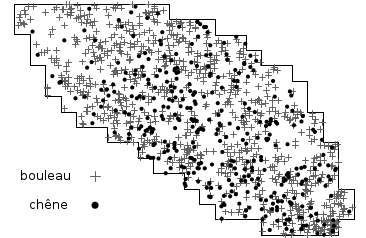
\includegraphics[scale=0.75]{images/diffPoints.png}
\end{minipage}


%%%%%%%%%%%%%%%%%%%%%%%%%%%%%%%%%%%%%%%%%%%%%%%%%%%%%%%%%%%%%%%%
\subsection{Répartition de point marqués}
\begin{minipage}{0.5\linewidth}
\indent
Marquer un point permet d'ajouter une information auxiliaire sur ce point (taille d'un arbre, masse d'une étoile)\\

La figure suivante montre par exemple la répartition d'arbre d'une forêt, et chaque arbre est représenté par un cercle plus ou moins gros en fonction de son diamètre en cm.
\end{minipage}\hfill
\begin{minipage}{0.5\linewidth}
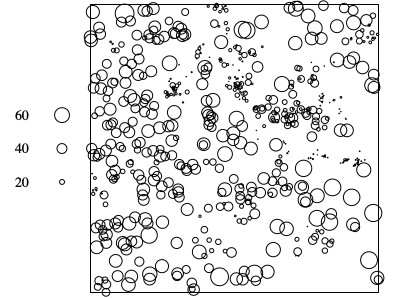
\includegraphics[scale=0.6]{images/pointsMarques.png}
\end{minipage}

%%%%%%%%%%%%%%%%%%%%%%%%%%%%%%%%%%%%%%%%%%%%%%%%%%%%%%%%%%%%%%%%
\subsection{Covariables}
\begin{minipage}{0.5\linewidth}
\indent
Les bases de données peuvent aussi inclure des covariables, c'est à dire des données utilisées pour expliquer un phénomène, plutôt que de répondre à une question.\\
La figure suivante montre par exemple la répartition d'arbre d'une forêt, avec une information d'altitude donnée en fond. Cette information n'est pas le but de l'étude, mais ajoute une explication possible.
\end{minipage}\hfill
\begin{minipage}{0.5\linewidth}
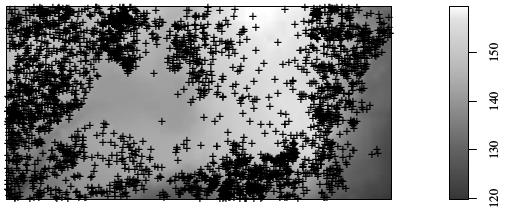
\includegraphics[scale=0.5]{images/covariables.png}
\end{minipage}
\\

%%%%%%%%%%%%%%%%%%%%%%%%%%%%%%%%%%%%%%%%%%%%%%%%%%%%%%%%%%%%%%%%
\subsection{Differentes dimensions spatiales}
Les localisations des points son généralement en 2 dimensions, mais on peut tout autant avoir une représentation spatiale en 1 dimension (accidents sur un réseau routier), en 3 dimensions (observation de cellules par un microscope 3D), ou même en espace-temps (localisation spatiale et temporel des épicentres de tremblement de terre).\\


%%%%%%%%%%%%%%%%%%%%%%%%%%%%%%%%%%%%%%%%%%%%%%%%%%%%%%%%%%%%%%%%
\subsection{Reproduction de répartitions}
On peut comparer des données prises à des données récoltés à des moment et endroits different pour en faire une analyse. Une reproduction d'expérience peut être traitée indépendemment ou bien apporter des informations suplémentaires à l'analyse d'une répétition d'exérience. Cela permet de séparer differentes sources de variables dans les expériences.\\

%%%%%%%%%%%%%%%%%%%%%%%%%%%%%%%%%%%%%%%%%%%%%%%%%%%%%%%%%%%%%%%

\section{Méthodes statistiques pour la répartition de point}

\subsection{Statistiques sommaires}
aaa\\

\subsection{Modèle statistique et inférence}
bbb\\

\subsection{Validation}
cc\\

%%%%%%%%%%%%%%%%%%%%%%%%%%%%%%%%%%%%%%%%%%%%%%%%%%%%%%%%%%%%%%%%
%%%%%%%%%%%%%%%%%%%%%%%%%%%%%%%%%%%%%%%%%%%%%%%%%%%%%%%%%%%%%%%%

\chapter{Correlation (chap. 7)}

\section{Introduction}

Le but de l'analyse d'une répartition de données ponctuelles est en général de déterminer si la position d'un points est indépendante ou non de celle d'un autre. Il y a alors 3 formes typiques de représentation:
\begin{itemize}
\item répulsif (points ont tous une certaine distance les uns des autres);
\item aléatoire (points n'ont pas de dépendance);
\item agrégée (points formes des groupes de points).\\
\end{itemize}

\begin{center} 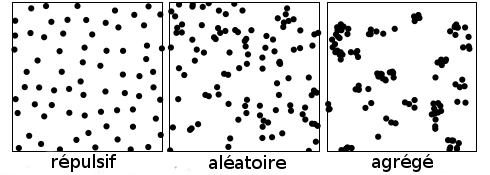
\includegraphics[scale=0.8]{images/repartition.png} \end{center}

Un outil standard pour mesurer cette dépendance est la covariance (2nd moment), c'est facile à calculer et à manipuler, mais cela requière une bonne estimation de la moyenne (1er moment) et cela ne permet pas de determiner le cause des regroupement de point (car c'est une statistique sommaire).

%%%%%%%%%%%%

\section{La fonction k}
\subsection{La fonction K empirique}
La fonction \begin{math}\hat{K}(r) \end{math} empirique est la moyenne cumulée des points se trouvant à une distance r de chaque point, corrigé pour les effets de bord et standardisé:
\begin{center}\begin{math} \hat{K}(r) = \mathbb{P}\{ d(u,X) \leq r \} \end{math}\end{center}
\subsection{La vraie fonction K d'un processus de point}
\subsection{Utilisation de la fonction K empirique}


\section{Correction des bords pour la fonction K}
\subsection{Estimation sans les effets de bords}
\subsection{Effets de bords}
\subsection{Correction des bords}
\subsection{Correction isotrope}
\subsection{Correction par translation}
\subsection{Discussion}

\section{Erreurs standard et interval de confiance}
\subsection{Variance sous CSR}
\subsection{Démarrage du system bloqué}
\subsection{Interval de confiance du syteme de démarrage de Loh}

\section{Tester si une répartition est complètement aléatoire}
\subsection{Enveloppes de point}
\subsection{Enveloppes globale}
\subsection{Tests non-graphiques}

%%%%%%%%%%%%%%%%%%%%%%%%%%%%%%%%%%%%%%%%%%%%%%%%%%%%%%%%%%%%%%%%
%%%%%%%%%%%%%%%%%%%%%%%%%%%%%%%%%%%%%%%%%%%%%%%%%%%%%%%%%%%%%%%%

\chapter{Espacement (chap. 8)}

\section{Introduction}
Les fonction statistique, telle que la fonction K, mesurant la correlation spatiale dans un processus de point sont des outils très populaire pour évaluer la dépendence. Cependant avec cette méthode, certain aspect de la dépendence ne peuvent être observés. Il faut alors utiliser les mesures sur les espaces ou les plus petites distances entre les points.

%%%%%%%%%%%%%%%%

\section{Fonction d'espace vide F}

\subsection{Définitions pour un processus de point stationnaire}
Si X est un processus de point spatial, la distance:
\begin{center}\begin{math} d(u,X) = min\{ ||u-x_i|| : x_i \in X \} \end{math}\end{center}
d'une position \begin{math} u \in \mathbb{R} \end{math} au plus proche point d'un processus est appelé 'distance d'espace vide'.\\
Pour un processus de point stationnaire, la fonction de distance d'espace vide est:
\begin{center}\begin{math} F(r) = \mathbb{P}\{ d(u,X) \leq r \} \end{math}\end{center}
définie pour toute distance \begin{math} r \geq 0 \end{math}, où u est une position quelconque.\\

Les valeurs de F(r) sont les probabilités (entre 0 et 1) pour n'importe quel point u, qu'il y ait un point X présent dans à une distance r ou moins de u (qu'il y ait un point dans le cercle de rayon r autour de u).\\

%%%%%%%%%%%%%%%%

\subsection{Valeurs pour un aléatoire complet}

\begin{minipage}{0.5\linewidth}
\indent
Pour un aléatoire complet, la fonction F suit une fonction de répatition de Poisson uniforme sur la surface d'un cercle (\begin{math} \pi r^2 \end{math}) soit pour une intensité \begin{math} \lambda \end{math} : 
\begin{center}\begin{math} F_{pois}(r) = 1 - exp(-\lambda \pi r^2) \end{math}\end{center}
C'est la fonction d'espace vide F théorique pour un aléatoire total.\\
\indent
La figure suivante montre la représentation en fonction de r de cette fonction théorique.
\end{minipage}\hfill
\begin{minipage}{0.5\linewidth}
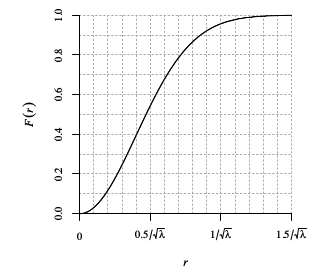
\includegraphics[scale=0.7]{images/poisson.png}
\end{minipage}

%%%%%%%%%%%%%%%%

\subsection{Interprétation de F}
La figure ci dessous montre la fonction estimé de F selon si la répartition est agrégée aléatoire ou bien répulsif. Les traits discontinues sont les représentation graphique de la fonction F théorique pour un aléatoire total.\\

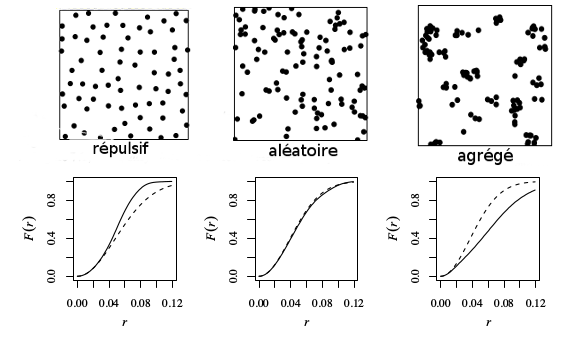
\includegraphics[scale=0.7]{images/interpret.png}

Sur la gauche, la courbe de la fonction calculée est au dessus de celle pour une répartition totalement aléatoire (\begin{math}\hat{F}(r) > F_p{pois}(r) \end{math}). Ainsi, pour une distance r, la probabilité que \begin{math} d(u,X) \leq r \end{math} est plus grande quelle ne l'est pour une répartition aléatoire, les espaces vides sont donc plus petits que prévu. Donc la répartition est répulsive.\\
\indent
Sur la droite, la courbe de la fonction calculée est en dessous de celle pour une répartition totalement aléatoire (\begin{math}\hat{F}(r) < F_p{pois}(r) \end{math}). Ainsi, pour une distance r, la probabilité que \begin{math} d(u,X) \leq r \end{math} est plus petite quelle ne l'est pour une répartition aléatoire, les espaces vides sont donc plus grands que prévu. Donc la répartition est agrégée.

%%%%%%%%%%%%%%%%%%%%%%%%%%%%%%%%%%%%%%%%%%%%%%%%%%%%%%%%%%%%%%%

\section{Fonction de plus proche voisins G}

\subsection{Définitions pour un processus de point stationnaire}
Si \begin{math}x_i\end{math} est un des points d'une représentation de points \textbf{x}, la distance du plus proche voisin de  \begin{math}x_i\end{math} est écrite telle que:
\begin{center}\begin{math} d_i = d(x_i,\textbf{x}\backslash x_i ) \end{math}\end{center}
la plus courte distance de \begin{math} x_i \end{math} à un autre point de \textbf{x} excepté \begin{math} x_i \end{math}.
Pour un processus de point stationnaire X, la fonction de distance du plus proch voisin est:
\begin{center}\begin{math} G(r) = \mathbb{P}\{ d(u,X\backslash u) \leq r | u \in X\} \end{math}\end{center}
définie pour toute distance \begin{math} r \geq 0 \end{math}, où u est une position quelconque.\\

%%%%%%%%%%%%%%%%

\subsection{Valeurs pour un aléatoire complet}

Pour un aléatoire complet, la fonction G est égale à la fonction d'espace vide F. Soit pour un un processus homogène de Poisson: 
\begin{center}\begin{math} G_{pois}(r) = 1 - exp(-\lambda \pi r^2) \end{math}\end{center}
Cela n'est vrai que pour une répartition totalement aléatoire, en général F et G seront des fonctions différentes.\\

%%%%%%%%%%%%%%%%

\subsection{Interprétation de G }
La figure ci dessous montre la fonction estimé de G selon si la répartition est agrégée aléatoire ou bien répulsif. Les traits discontinues sont les représentation graphique de la fonction F théorique pour un aléatoire total.\\

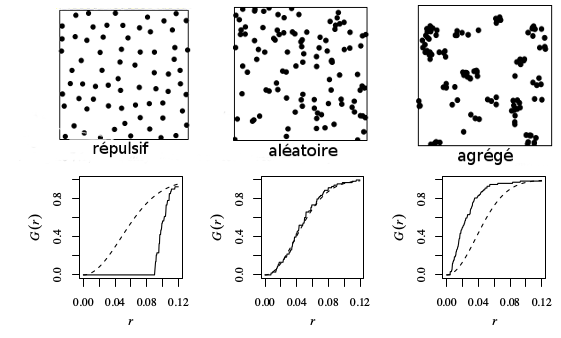
\includegraphics[scale=0.7]{images/interpret2.png}

Sur la gauche, la courbe de la fonction calculée est en dessous de celle pour une répartition totalement aléatoire (\begin{math}\hat{G}(r) < G_p{pois}(r) \end{math}). Ainsi, les distances des plus proches voisins sont plus grandes que celles prévues pour une répartiton aléatoire. Donc la répartion est répulsive.\\
\indent
Sur la droite, la courbe de la fonction calculée est au dessus de celle pour une répartition totalement aléatoire (\begin{math}\hat{G}(r) > G_p{pois}(r) \end{math}). Ainsi, les distances des plus proches voisins sont plus petites que celles prévues pour une répartiton aléatoire. Donc la répartion est agrégée.\\


\section{Intervals de confiance et enveloppes de simulation}

\section{Hasard de l'espace vide (désavantages)}

%%%%%%%%%%%%%%%%
\section{Fonction J}

Les distances du plus proche voisin et les distances d'espace-vide ont la même distribution de probabilité si la répartition des point est totalement aléatoire. Pour les départs des expériences avec une répartission aléatoire complète, ces distances ont tendance à répondre dans des directions opposées: l'un devient plus grand et l'autre plus petit. Cela suggère qu'une comparaison de ces 2 types de distance pourrait s'avérer utile pour évaluer les départ d'une répartion aléatoire.\\

Une combinaison pratique de G et F, suggérée par la théorie fondamentale, est la fonction J d'un processus stationnaire ponctuel:
\begin{center}\begin{math} J(r) = \frac{1-G(r)}{1-F(r)} \end{math}\end{center}
définie pour tout \begin{math} r \geq 0 \end{math} telle que F(r)<1. Pour un processus de Poisson homogène, \begin{math} F_{pois} \equiv G_{pois} \end{math} ainsi les valeures de J(r) > 1 son cohérent avec une représentation répulsive, tandis que les valeures de J(r) < 1 sont cohérente avec une représentation agrégée.

La fonction J empirique est insemsible aux effets de bords, car ceux-ci s'annulent dans le ratio (1 - G)/(1 - F).

%%%%%%%%%%%%%%%%

\section{Théorie pour la correction des bords}
\subsection{Estimation de F et G sans effets de bord}
\subsection{Effets de bords pour F et G}
\subsection{Correction des bords}
\subsection{Correction de Kaplan-Meier}
\subsection{Correction de Hanisch-Chiu-Stoyan}
\subsection{Comparaison des méthodes}



\end{document}
